% !TeX TXS-program:compile = txs:///pdflatex/[-shell-escape]
\documentclass[xcolor=table]{beamer}

\mode<presentation> {

% The Beamer class comes with a number of default slide themes
% which change the colors and layouts of slides. Below this is a list
% of all the themes, uncomment each in turn to see what they look like.

\usetheme{default}
%\usetheme{AnnArbor}
%\usetheme{Antibes}
%\usetheme{Bergen}
%\usetheme{Berkeley}
%\usetheme{Berlin}
%\usetheme{Boadilla}
%\usetheme{CambridgeUS}
%\usetheme{Copenhagen}
%\usetheme{Darmstadt}
%\usetheme{Dresden}
%\usetheme{Frankfurt}
%\usetheme{Goettingen}
%\usetheme{Hannover}
%\usetheme{Ilmenau}
%\usetheme{JuanLesPins}
%\usetheme{Luebeck}
%\usetheme{Madrid}
%\usetheme{Malmoe}
%\usetheme{Marburg}
%\usetheme{Montpellier}
%\usetheme{PaloAlto}
%\usetheme{Pittsburgh}
%\usetheme{Rochester}
%\usetheme{Singapore}
%\usetheme{Szeged}
%\usetheme{Warsaw}

% As well as themes, the Beamer class has a number of color themes
% for any slide theme. Uncomment each of these in turn to see how it
% changes the colors of your current slide theme.

%\usecolortheme{albatross}
%\usecolortheme{beaver}
%\usecolortheme{beetle}
%\usecolortheme{crane}
%\usecolortheme{dolphin}
%\usecolortheme{dove}
%\usecolortheme{fly}
%\usecolortheme{lily}
%\usecolortheme{orchid}
%\usecolortheme{rose}
%\usecolortheme{seagull}
%\usecolortheme{seahorse}
%\usecolortheme{whale}
%\usecolortheme{wolverine}
%\setbeamertemplate{footline} % To remove the footer line in all slides uncomment this line
\setbeamertemplate{footline}[page number] % To replace the footer line in all slides with a simple slide count uncomment this line

\setbeamertemplate{navigation symbols}{} % To remove the navigation symbols from the bottom of all slides uncomment this line 
}




%\setlength {\textwidth}{16.5truecm} 
%{\textheight}{22.0truecm} \calclayout
\usepackage{amsmath} 
\usepackage{graphicx} % Allows including images
\usepackage{booktabs} % Allows the use of \toprule, \midrule and \bottomrule in tables

\usepackage[table]{xcolor}

\usepackage{mathrsfs}


\usepackage{tikz}

\usepackage{pstricks-add}
\usetikzlibrary{arrows,shapes,positioning,shadows,patterns,trees}

\usepackage{tcolorbox}
\usepackage{wrapfig}
\usepackage{subfig}
\usepackage{hyperref}
\hypersetup{
    colorlinks,
    citecolor=black,
    filecolor=black,
    linkcolor=black,
    urlcolor=black
}
\newcommand{\notimplies}{%
    \mathrel{{\ooalign{\hidewidth$\not\phantom{=}$\hidewidth\cr$\implies$}}}}


\DeclareMathAlphabet\mathzapf{T1}{pzc}{mb}{it}
\usepackage{amsmath,wasysym}
\usepackage{latexsym}

\usepackage{amssymb}
\usepackage{mathrsfs}
\usepackage{wrapfig}
\usepackage{fancybox}
\bibliographystyle{amsplain}
\usepackage{systeme}
\usepackage{pdfpages}
\usepackage{pgfplots}
\usepackage{tcolorbox}
\pgfplotsset{compat=1.15}


\usepackage{yfonts}
\usepackage[french]{babel}



\usepackage[T2A]{fontenc}





%\usepackage[style=ieee]{biblatex} %Use if necessary for citation
%\addbibresource{biblatex-examples.bib}
%----------------------------------------------------------------------------------------
%	TITLE PAGE
%----------------------------------------------------------------------------------------

\title[Physique]{Mathématiques II} % The short title appears at the bottom of every slide, the full title is only on the title page

\author{Team Physique} % Your name
\institute[S4S] % Your institution as it will appear on the bottom of every slide, may be shorthand to save space
{
initiative S4S\\ % Your institution for the title page
\medskip
}
\date{\today} % Date, can be changed to a custom date
\begin{document}

\begin{frame}
\titlepage % Print the title page as the first slide
\end{frame}

\begin{frame}{Approximation et développements limités}

\begin{figure}[ht]

\begin{center}
\definecolor{ccqqqq}{rgb}{0.8,0,0}
\definecolor{qqqqff}{rgb}{0,0,1}
\begin{tikzpicture}[line cap=round,line join=round,>=triangle 45,x=1cm,y=1cm]
\begin{axis}[
x=1cm,y=1cm,
axis lines=middle,
xmin=-2.5400689538405253,
xmax=2.536515566558789,
ymin=-2.111629827594053,
ymax=2.178011872488389,
xtick={-2,-1,...,2},
ytick={-2,-1,...,2},]
\clip(-2.8400689538405253,-2.111629827594053) rectangle (3.136515566558789,2.478011872488389);
\draw[line width=0.8pt,color=qqqqff,smooth,samples=100,domain=-2.8400689538405253:3.136515566558789] plot(\x,{cos(((\x))*180/pi)});
\draw [line width=0.8pt,color=ccqqqq,domain=-2.8400689538405253:3.136515566558789] plot(\x,{(--1-0*\x)/1});
\end{axis}
\end{tikzpicture}
%
\definecolor{ccqqqq}{rgb}{0.8,0,0}
\definecolor{qqqqff}{rgb}{0,0,1}
\begin{tikzpicture}[line cap=round,line join=round,>=triangle 45,x=1cm,y=1cm]
\begin{axis}[
x=1cm,y=1cm,
axis lines=middle,
xmin=-2.5400689538405253,
xmax=2.536515566558789,
ymin=-2.111629827594053,
ymax=2.178011872488389,
xtick={-2,-1,...,2},
ytick={-2,-1,...,2},]
\clip(-2.4558532849474526,-1.8811746892214536) rectangle (2.7186787673463244,2.092541068425681);
\draw[line width=0.8pt,color=qqqqff,smooth,samples=100,domain=-2.4558532849474526:2.7186787673463244] plot(\x,{sin(((\x))*180/pi)});
\draw [line width=0.8pt,color=ccqqqq,domain=-2.4558532849474526:2.7186787673463244] plot(\x,{(-0--1*\x)/1});
\end{axis}
\end{tikzpicture}
\end{center}

\caption{Approximation linéaire du cosinus (à gauche) et du sinus (à droite) autour de $0$}
    \label{fig:dl}
\end{figure}
\end{frame}

\begin{frame}{Approximation et développements limités : }
    

%Dessin de l'approximation
\begin{figure}
    
    
\definecolor{ffqqqq}{rgb}{1,0,0}
\definecolor{qqqqff}{rgb}{0,0,1}
\begin{center}

\begin{tikzpicture}[line cap=round,line join=round,>=triangle 45,x=1cm,y=1cm,scale=0.5
]
\begin{axis}[
x=2cm,y=1cm,
axis lines=middle,
xmin=-3.780437787628234,
xmax=4.220977016145955,
ymin=-3.0784578863074157,
ymax=3.0661263520169277,
xtick={-3.5,-2.5,...,3.5},
ytick={-3,-2,...,3},]
\clip(-3.780437787628234,-3.0784578863074157) rectangle (4.220977016145955,3.0661263520169277);

\draw[line width=0.8pt,color=red,smooth,samples=100,domain=-3.780437787628234:4.220977016145955] plot(\x,{(\x)});
\draw[line width=0.8pt,color=green,smooth,samples=100,domain=-5.1874758166367645:5.462407287186683] plot(\x,{(\x)-(\x)^(3)/6});
\draw[line width=0.8pt,color=yellow,smooth,samples=100,domain=-5.660273317658524:6.05459809654727] plot(\x,{(\x)-(\x)^(3)/6+(\x)^(5)/120});
\draw[line width=1pt,color=blue,smooth,samples=100,domain=-3.780437787628234:4.220977016145955] plot(\x,{sin(((\x))*180/pi)});
\begin{scriptsize}

\end{scriptsize}
\end{axis}
\end{tikzpicture}
\end{center}


\caption{Approximation de la fonction sinus avec de polynômes de Taylor de différents degré}
    \label{fig:my_label}
\end{figure}

\end{frame}

\begin{frame}{Equations différentielles: Exemple d'application (2)}
    \begin{figure}[H]
    \centering
    \subfloat{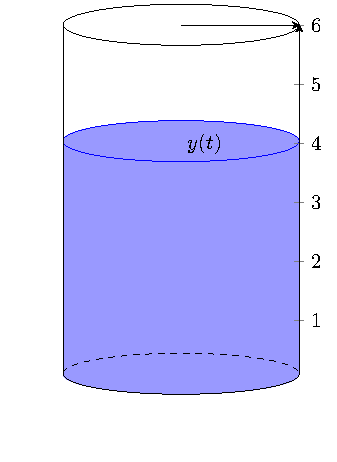
\includegraphics[scale=0.85]{Images/cyl1.pdf}}
    \hfill
    \subfloat{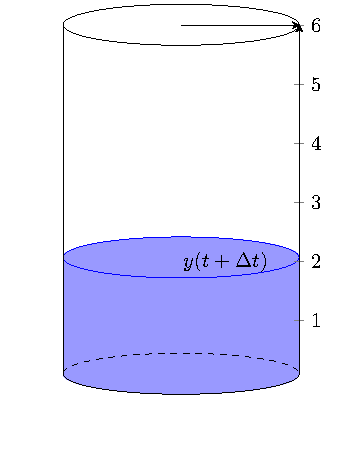
\includegraphics[scale=0.85]{Images/cyl2.pdf}}
    \caption{Niveau d'eau d'un cylindre qui fuit}
    \label{fig:cyl}
\end{figure}
\end{frame}
\begin{frame}{Equations différentielles :}

 
\begin{figure}[H]
   \centering
  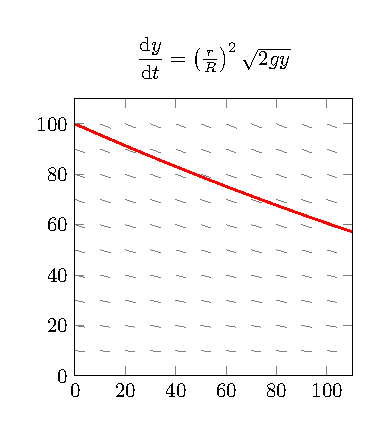
\includegraphics[scale=0.85]{Images/dif1.pdf}
    \caption{Le niveau d'eau dans le temps d'un réservoir qui fuit dépend de sa taille}
    \label{fig:dif2}

\end{figure}
\end{frame}

\end{document}